\subsection{Video Playback Model}\label{sec:application:qoe_user_behaviour:system_model}
This section provides a system model for video playback, in order to study the stalling behaviour of \gls{HTTP} video streaming.
We consider the playback of a video consisting of multiple frames, as shown in \reffig{fig:application:qoe_user_behaviour:system_model:steady_state:player}.
The frames are downloaded in-order and arrive at the client with rate \(\lambda\) while the playback time is given by the video framerate \(\mu\), resulting in an offered load of \(a = \frac{\lambda}{\mu}\). Here, \(a\) quantifies the available network bandwidth normalised by the video framerate. We assume a stable system, i.e. that \(a < 1\) holds.
In order to reduce the number of stalling events during playback, the video player uses a playback buffer.
Video playback stops, if less than \(q\) frames are currently available for playback and is only resumed if the buffer contains \(p = q + d\) frames. 
The normalised buffer size \(d^*\), in video seconds, relates the buffer size \(d\), which is given in frames, to the video framerate \(\mu\), i.e. \(d^*=\frac{d}{\mu}\).

Next, we introduce metrics used to evaluate the influence of the playback buffer parameter selection.
The relative amount of time spent in stalling compared to the total duration of the playback process including stalling is given by the stalling ratio \stallingRatio and the number of stalling events normalised by the video length \(N^*\).
For the case of finite videos we furthermore consider the stalling duration \stallingDuration which gives the sum of times spent in stalling states during the complete video playback. 


\subsubsection*{\(M/M/1\) Queue with \(pq\)-Policy}\label{sec:application:qoe_user_behaviour:system_model:mm1pq}
The state of the video playback is characterised by the tuple \((i, j)\), where \(i \in \{0, 1\}\) is the playback state of the client, i.e. the video is not played back if \(i\) is \(0\) and the video is played back if \(i\) is \(1\).
Furthermore, \(j \geq 0\) gives the number of unplayed frames currently available at the client.
Furthermore, we give the probability of the playback being in state \((i, j)\) as \(x(i, j)\).

\begin{figure}
  \centering
  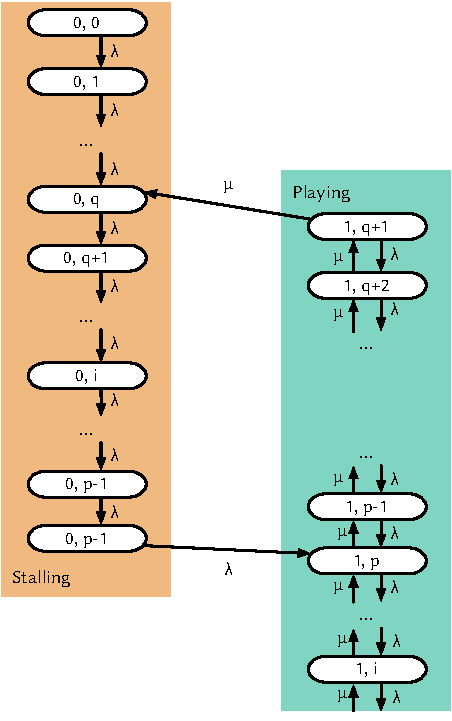
\includegraphics{application/qoe_user_behaviour/system_model/figures/state_diagram}
  \caption{System model for the \(M/M/1\) queue with \(pq\)-policy.}
  \label{fig:application:qoue_user_behaviour:system_model:mm1pq:state_diagram}
\end{figure}


We obtain the following equilibrium state equations, based on the state diagram given in \reffig{fig:application:qoue_user_behaviour:system_model:mm1pq:state_diagram}.
\begin{align*}
  \lambda x(0, 0) &= 0 & &\\
  \lambda x(0, i) &= \lambda x(0, i-1) & i&\in \left[1, q\right)\\
  \lambda x(0, q) &= \lambda x(0, q-1) + \mu x(1, q+1) & &\\
  \lambda x(0, i) &= \lambda x(0, i-1) & i&\in\left(q, p\right)\\
  (\lambda + \mu) x(1, q+1) &= \mu x(1, q+2) & &\\
  (\lambda + \mu) x(1, i) &= \lambda x(1, i-1) + \mu x(1, i+1) & i&\in\left(q+1, p\right)\\
  (\lambda + \mu) x(1, p) &= \lambda (x(0,p-1) + x(1, p-1)) & &\\
  & + \mu x(1, p+1) & &\\
  (\lambda + \mu) x(1, i) &= \lambda x(1, i-1) + \mu x(1, i+1) & i&\in\left(p, +\infty\right)
\end{align*}
State probabilities are obtained using macro state equations and recursive reduction and follow analogously to~\cite{Zhang2004}:
\begin{align*}
x(0, i) &= 0 & i&\in \left[0,q\right)\\ 
x(0, i) &= \frac{1-a}{d} &i&\in \left[q,p\right)\\
x(1, i) &= \frac{a(1- a^{i-q})}{d} &i&\in \left(q,p\right]\\
x(1, i) &= \frac{a^{j-p+1}(1-a^{d})}{d} &i&\in \left(p,+\infty\right]
\end{align*}

From this, we obtain the stalling ratio \stallingRatio as the probability of being in a stalling state, i.e.
\begin{equation}
\stallingRatio = \sum_{i=0}^{p-1} x(0, i) = 1-a \, .
\label{eq:application:qoe_user_behaviour:system_model:mm1pq:stalling_ratio_queuing}
\end{equation}

\subsubsection*{Mean Value Analysis of Steady State}\label{sec:application:qoe_user_behaviour:system_model:steady_state}
While the \(M/M/1-pq\) model provides results for infinite length videos, real-world videos however are of finite length.
This requires the study of additional metrics, i.e. the number of stalling events during playback \numberStallingEvents.
Thus, in this section we derive a mean value analysis of the proposed video playback model according to \reffig{fig:application:qoe_user_behaviour:system_model:steady_state:player}.

\begin{figure}
  \centering
  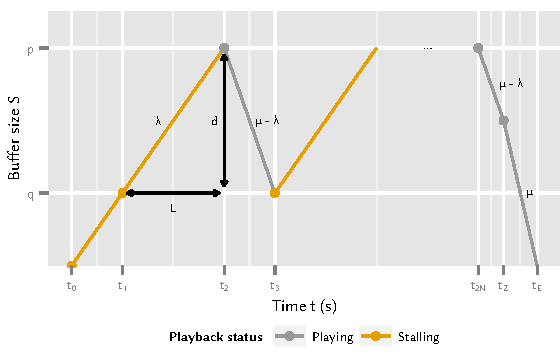
\includegraphics{application/qoe_user_behaviour/system_model/figures/player}
  \caption{Video buffer status evolving over time with constant video bit rate \(\mu\) and network bandwidth for a finite video of duration \(T\) and \(Z\) frames.}
  \label{fig:application:qoe_user_behaviour:system_model:steady_state:player}
\end{figure}

Assuming that the initial download begins at \(t_0\) and new frames arrive with rate \networkBandwidth at the client.
The number of frames in the buffer \currentNumberFrames exceeds \(q\) the first time at \(t_1\).
At time \(t_2\), the threshold of \(p\) is reached for the first time and playback begins.
While the download of new frames continues with rate \networkBandwidth, frames are played out with rate \playbackRate, resulting in a buffer change with rate \(\playbackRate - \networkBandwidth\).
Thus, the number of buffered frames \currentNumberFrames reaches \(q\) at time \(t_3\).
This process repeats, resulting in an alternating chain of stalling and playback phases.

In this analysis, we consider the steady state, i.e. especially neglecting the time \(t_1 - t_0\).
First, we consider the time required for the buffer to fill from \(q\) frames to \(p\) frames, i.e. obtaining \(d\) frames while no playback is occurring.
This time depicts the average duration \(\meanStallingEventDuration\) of a single stalling event.

In \reffig{fig:application:qoe_user_behaviour:system_model:steady_state:player} this is given as the time between \(t_1\) and \(t_2\), and we get
\begin{equation*}
L=t_2-t_1 = \frac{p-q}{\lambda}=\frac{d}{\lambda} = \frac{d^*}{a}\, .
\end{equation*}
The average stalling length \(\meanStallingEventDuration\) only depends on the actual buffer size \(d\) and the network bandwidth \(\networkBandwidth\).

Next, we consider the time required for the number of frames \currentNumberFrames in the buffer to decrease from \(p\) 
to \(q\), i.e. the time between \(t_2\) and \(t_3\), 
\[t_3-t_2 = \frac{d}{\mu-\lambda},\]
which represents the time of uninterrupted playback between each stalling event.

Combining these two equations we get the time between two stalling event as
\[
t_3-t_1=(t_3-t_2)+(t_2-t_1)=\frac{\mu d}{(\mu-\lambda)\lambda}.
\]

The stalling ratio \stallingRatio follows as
\begin{equation*}
\stallingRatio = \frac{t_2-t_1}{t_3-t_1} = 1-a,
\end{equation*}
yielding the same result as in \refeq{eq:application:qoe_user_behaviour:system_model:mm1pq:stalling_ratio_queuing}.

Finally, we can obtain the number of of stalling events normalised by video duration by analysing the busy periods of the system.
Here, the mean idle period is given by \(\meanIdle = \frac{d}{\lambda}\).

For the mean busy period \(\meanBusy\) we obtain
\[
\frac{\meanBusy}{\meanBusy + \meanIdle} = 1 - R = a \, ,
\]
which yields
\[
\meanBusy = \frac{a}{1-a}\frac{\lambda}{d} 
\]
and in turn can be used to obtain the normalised number of stalling events 
\begin{equation*}
N^* = \frac{1}{\meanBusy}=\frac{\mu-\lambda}{d} = \frac{1-a}{d^*}\, .
\end{equation*}

This equation can also be derived by considering \(N^*=\frac{1}{t_3-t_2}\). 
While \(N^*\) relates the number of stalling events to the video duration, the stalling frequency \(F\) denotes the number of stalling events per unit time. 
It holds \(F=\frac{1}{t_3-t_1}=a N^*\) which can be obtained as \(F=x(0,p-1) \lambda\) to weight the state probability of player state change \(x(0,p-1)\) with the network arrival rate \(\lambda\). 
From an end user's point of view, the metric $N^*$ is of higher importance. 

Beside the network bandwidth \(\lambda\) and the video bit rate \(\mu\), the metric \(N^*\) of stalling events depends only on the video buffer size \(d=p-q\), but not on the concrete values of \(p\) and \(q\) in the steady state.


\subsubsection*{Mean Value Analysis of Finite Videos and User Aborts}\label{sec:application:qoe_user_behaviour:system_model:finite_video}

As we will see later in \refsec{sec:application:qoe_user_behaviour:typical_user_scenarios}, the steady state analysis is sufficient to dimension the buffer. 
However, in practice, playback is finite, as either the video is of finite length \(T\), or due to the fact that a user aborts playback after a number of \(T\) seconds.
This behaviour is shown in \reffig{fig:application:qoe_user_behaviour:system_model:steady_state:player}.

We do not consider the time until the initial playback, i.e. the time between \(t_0\) and \(t_2\) as stalling, since it has a much lower impact on the perceived quality than stalling \cite{Garcia2014} and it only depends on the network bandwidth \networkBandwidth and thus is not subject to optimisation.
First, we consider the case where the user plays back the complete video.
Given the network bandwidth \networkBandwidth and a video of \numberFrames Frames, the required download time for the complete video is \(\videoDownloadTime = \frac{Z}{\lambda}\).
Within \videoDownloadTime there are \(N\) phases of stalling and playback and each phase is of duration \(t_3 - t_1\), i.e.
\[
N = \left\lfloor \frac{t_Z-t_1+t_0}{t_3-t_1} \right\rfloor .
\]

Next, we consider the case where the user aborts playback of the video after \(T\) seconds of video have been watched.
Here, the number of stalling phases is given as 
\[
N = \left \lfloor{T / (t_3 - t_2)}\right \rfloor,
\]
rounding down as we do not consider the initial delay before playback as stalling.
Again, we can obtain the number of stalling events normalized by video length as
\(N^*=\frac{N}{T}\).